\section{Massive and Artifact Tokens}
\label{sec:artifact_tokens}



\subsection{Notation}
While vision transformers may vary in architecture, most such as CLIP and DINO employ the one proposed by \cite{dosovitskiy2021vit}. We represent a tokenized image as a sequence of $N$ input embeddings $\emb{0}{1}, \emb{0}{2}, \ldots, \emb{0}{N} \in \R^D$ along with the class (CLS) token $\emb{0}{CLS}$, which are vertically stacked to compose $\Emb{0} = \tr{[\emb{0}{CLS} \quad \emb{0}{1} \quad \cdots \quad \emb{0}{N}]} \in \R^{(N + 1) \times D}$. For ease of notation, $\emb{\ell}{0}$ will be equivalent to $\emb{\ell}{CLS}$. Throughout the paper, layers, both as part of equations and explicitly referred to, will be zero-indexed. We define an $L$-layer transformer to be a sequence $(\lyr{0}, \ldots, \lyr{L - 1})$ where $\lyr{\ell}$ is equipped with the $4$-tuple of functions $(\lyn{1}{\ell}, \attn{\ell}, \lyn{2}{\ell}, \mlp{\ell})$, and \begin{alignat}{3}
    & \Emb{\ell + 1/2}  && = \Emb{\ell} + \attn{\ell}(\lyn{1}{\ell}(\Emb{\ell})), \label{eqn:layer}   \\
    & \Emb{\ell + 1}    && = \Emb{\ell + 1/2} + \mlp{\ell}(\lyn{2}{\ell}(\Emb{\ell + 1/2})), \\
    & \Emb{\ell + 1}    && = \lyr{\ell}(\Emb{\ell}).
\end{alignat} Although each of these four functions are parameterized by some set of learned weights, our analysis is primarily concerned with those composing the attention operation. In a multi-head attention operation with $H$ distinct heads, these weights are denoted as $\cbn{(\Ql{\ell}_h, \Kl{\ell}_h, \Vl{\ell}_h, \Olw{\ell}{h})}_{h \in [H]}$ and $\Olb{\ell}$ where $H \cdot d = D$, $\Ql{\ell}_h, \Kl{\ell}_h, \Vl{\ell}_h: \R^D \to \R^{d}$, $\Olw{\ell}{h} \in \R^{D \times d}$, and $\Olb{\ell} \in \R^D$. For the sake of brevity, $\Ql{\ell}_h(\lyn{1}{\ell}(\Emb{\ell}))$ can be abbreviated as $\Ql{\ell}_h \in \R^{(N + 1) \times d}$, with $\Kl{\ell}_h$ and $\Vl{\ell}_h$ being abbreviated identically. Where $\Embp{\ell} = \lyn{1}{\ell}(\Emb{\ell})$, the attention operation is given by \begin{align}
    \attn{\ell}(\Embp{\ell}) = \Olb{\ell} + \dss{h}{} \sf\pfrac{\Ql{\ell}_h{\mbf{K}^{(\ell)\top}_h}}{\sqrt{d}}\Vl{\ell}_h{\mbf{O}^{(\ell)\top}_{h, weight}}, \label{eqn:attn}
\end{align} where $\sf$ denotes the softmax operator, which will only refer to its application on the last dimension to avoid ambiguity in cases where its operand tensor has more than one dimension. For an attention matrix $\Al{\ell}_h = \sf(\Ql{\ell}_h{\mbf{K}^{(\ell)\top}_h} / \sqrt{d})$, we primarily employ the indexing notation $\Al{\ell}_{h, i \to j}$ to emphasize that that entry represents the attention from $i$ to $j$.





\subsection{Attention Sinks}
\label{sec:attention_sinks}
\begin{figure*}[t]
    \centering
    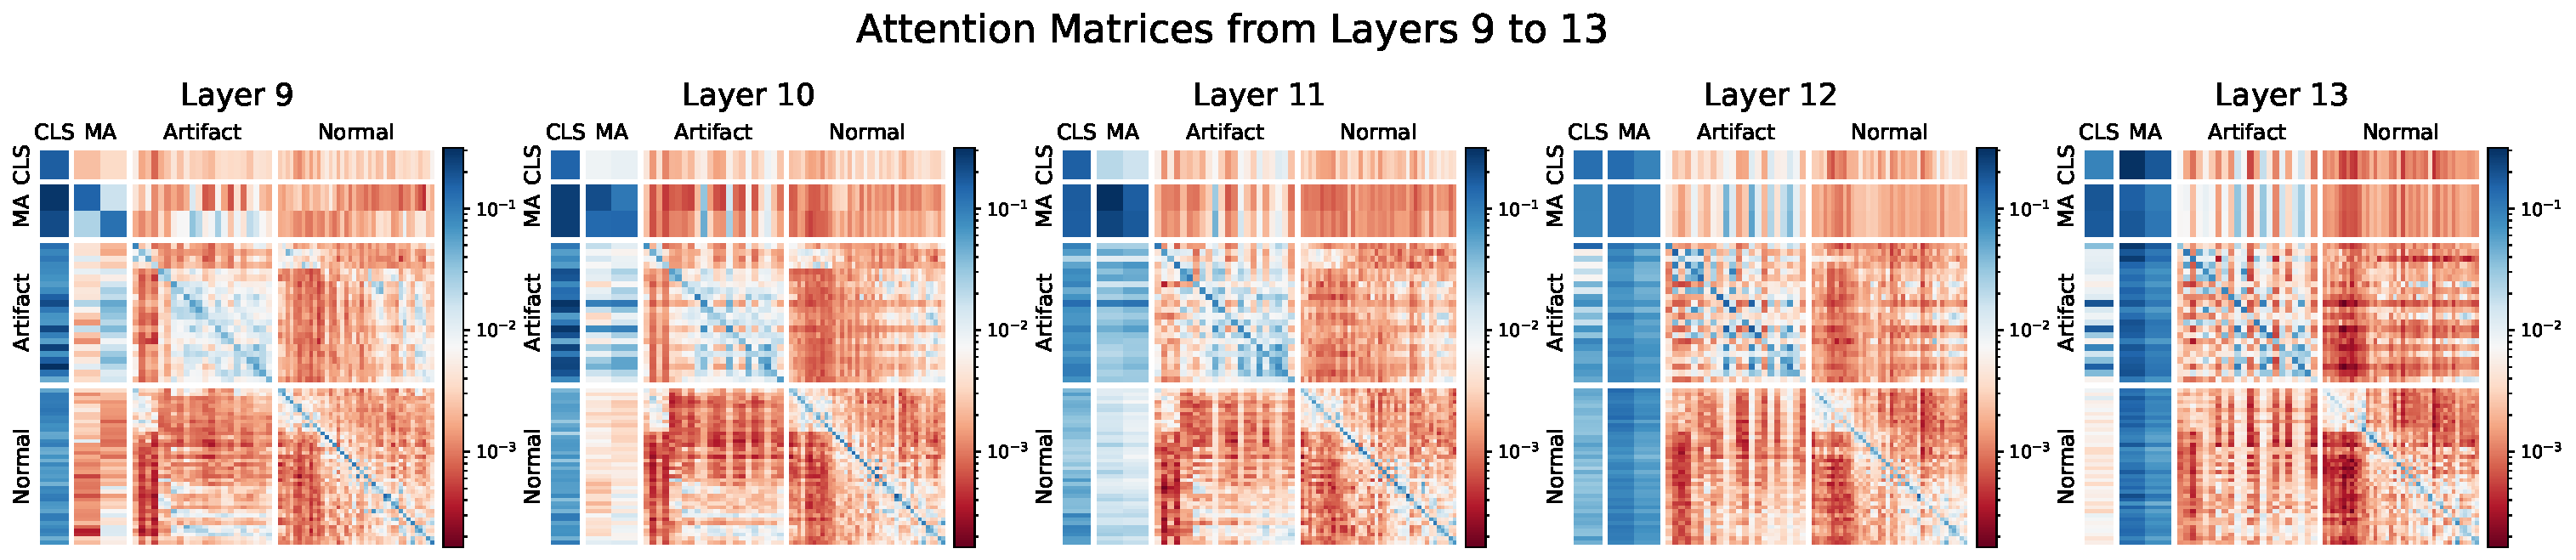
\includegraphics[width=1\linewidth]{figs/attention_transition_L9toL13.pdf}
    \vspace{-1.5em}
    \caption{Each subplot visualizes the mean attention matrix across heads for a single image at a particular layer of CLIP ViT L-14. In an image tokenization with $256$ image tokens and one CLS token, the mean attention matrix is $257 \times 257$ which is difficult to visualize. We permute the order of tokens and resize sections of the attention matrix to distinguish small subsets of tokens that are of interest, particularly massive tokens, and artifact tokens. Additionally, we subsample a portion of the remaining tokens which allows us to see them in detail as well as eliminate any perceptive bias resulting from the discrepancy in scale. We can see that in layers 9 and 10, massive tokens are characterized by large attention to the CLS token and large attention to itself, and become attention sinks in layers 11 to 13 where they attract a large proportion of attention from all tokens.}
    \label{fig:attention_transition_layers}
\end{figure*}

While massive tokens are most easily observed through their large activation norms, they also attract a large proportion of attention from all tokens. We find that the constitution of a large proportion of attention within very few tokens is critical to generating effective feature representations; however, their presence in later layers modestly detracts accumulation of information into the class (CLS) token. As seen in Figure \ref{fig:dino_clip_artifacts}, the denoising of such tokens improves the quality and coherency of feature representations in the final layers.

We also observe that the incoming attention to massive tokens dramatically increases over their formative layers as seen in Figure \ref{fig:attention_transition_layers}. Though the massive tokens that emerge naturally from a model number very few (approximately 2-3 per image), we find that models actually learn a robust process that enables other suitable tokens to become massive in their place should the original massive tokens be removed. Furthermore, those tokens are roughly ordered, in which a suitable token will become massive only if a sufficient set of tokens that precede it have been removed via masking. We denote these dormant tokens as \textit{artifact tokens}, and the pool of (potential) massive tokens as a whole as \textit{attention sinks}. Any image (non-CLS) token that is neither a massive token nor artifact token is referred to as a \textit{normal token}.

Since attention sinks serve a critical role in attracting attention, extracting such tokens can be intuitively performed by thresholding their average incoming attention after formation. However, we also find that attention \textit{from} the CLS token provides a more distinct signal for determining attention sinks. Specifically, we select a detection layer $\ld$ such that if $\Al{\ld} \in \R^{(N + 1) \times (N + 1)}$ represents the mean attention matrix in layer $\ld$, then token $t$ is labeled an attention sink if $\Al{\ld}_{CLS \to t} \geq \Al{\ld}_{CLS \to CLS}$, i.e. if the mean attention from CLS to $t$ exceeds the mean attention from CLS to itself.

This detection layer is typically $13$ for CLIP and $20$ for DINOv2 ViT L-14. While not all massive tokens meet the CLS threshold, it is also true that not all potential massive tokens exhibit immediate largeness or attention-sinkness. Therefore,  this observation alone does not suggest a method that is able to determine all such tokens within one iteration. In Section \ref{sec:iterative_masking}, we discuss an iterative procedure based on this intuition for determining both the set of attention sink tokens and their priority order. Additionally, in Section \ref{sec:artifact_classifier}, we present a fast, non-iterative method that is able to determine the set of attention sink tokens alone.


% We can see in Figure \ref{fig:CLS_attention_proxy} that attention from the CLS token serves as a good proxy from mean incoming attention. While it is clear from the figure that not all massive tokens meet the CLS threshold, not all potential massive tokens exhibit immediate largeness or attention-sinkness anyways, so this observation alone does not suggest a method that is able to determine all such tokens within one iteration. We discuss in \ref{sec:iterative_masking} the iterative procedure based on this intuition for determining both the set of attention sink tokens and their order of priority, and in \ref{sec:artifact_classifier} a fast, non-iterative method that is able to determine the set of attention sink tokens alone.

% \begin{figure}[H]
%     \centering
%     \includegraphics[width=1\linewidth]{figs/attention_to_CLS_proxy.pdf}
%     \caption{The $x$-axis shows the mean incoming attention to a token, both across heads and across query tokens, which quantifies attention-sinkness. The $y$-axis shows the mean attention from the CLS token, normalized by the mean attention from the CLS token to itself. This normalization allows us to visualize the same thresholding across multiple images, which may have different CLS-to-CLS attentions. Thus, surpassing the normalized threshold of $1$ indicates that a token under the current configuration of masking is considered an attention sink.}
%     \label{fig:CLS_attention_proxy}
% \end{figure}



\subsection{Iterative Detection of Attention Sinks}



\label{sec:iterative_masking}
Our iterative procedure is formalized to extract all (potential) attention sinks. While the pseudocode (Algorithm \ref{alg:iterative_sink_detection}) is provided in concrete detail pertaining to CLIP ViT L-14, an analogous method can be applied to other vision transformers.
\begin{algorithm}[H]
    \caption{Attention Sink Detection via Iterative Removal}
    \hspace*{\algorithmicindent} \textbf{Input:} $\Emb{0} \in \R^{(N + 1) \times D}$ \\
    \hspace*{\algorithmicindent} \textbf{Output:} List $\mc{T} = (t_1, t_2, \ldots) \subseteq [N]$ of attention sinks.
    \begin{algorithmic}[1]
        \Procedure{ComputeSinks}{$\Emb{0}$}
            \State $\lm, \ld \gets 9, 13$
            \State Run transformer layers $0$ to $\lm - 1$
            \State Initialize $\mc{T}$ as $\emptyset$
            \While{$\mc{T}$ has not converged}
                \State Rerun $\lm$ to $\ld$ masking $\mc{T}$
                \State Let $A$ be the mean attention matrix at $\ld$
                \State Append $t$ to $\mc{T}$ if $A_{CLS \to t} > A_{CLS \to CLS}$
            \EndWhile
            \State \Return $\mc{T}$
        \EndProcedure
    \end{algorithmic}
    \label{alg:iterative_sink_detection}
\end{algorithm}
\vspace{-8pt}
% \begin{algorithm}[H]
%     \caption{Attention Sink Detection via Iterative Removal}
%     \hspace*{\algorithmicindent} \textbf{Input:} $\Emb{0} \in \R^{(N + 1) \times D}$ \\
%     \hspace*{\algorithmicindent} \textbf{Output:} List $\mc{T} = (t_1, t_2, \ldots) \subseteq [N]$ of attention sinks.
%     \begin{algorithmic}[1]
%         \Procedure{ComputeSinks}{$\Emb{0}$}
%             \State $\lm, \ld \gets 9, 13$
%             \State 
%             \For{$0 \leq \ell < \lm$}
%                 \State $\Emb{\ell + 1} \gets \lyr{\ell}(\Emb{\ell})$
%             \EndFor
%             \State $\mc{T}, \mc{T}' \gets \emptyset, \cbn{-1}$
%             \While{$\absn{\mc{T}'} > 0$}
%                 \For{$\lm \leq \ell < \ld$}
%                     \State $\Emb{\ell + 1} \gets \lyrm{\ell}(\Emb{\ell}, M_I(\mc{T}))$
%                 \EndFor
%                 \State $\Wl{\ld}_h \gets \Ql{\ld}_h{\mbf{K}^{(\ld)\top}_h} / \sqrt{d}$
%                 \State $\Al{\ld} \gets \frac{1}{H} \dss{h}{} \sfm(\Wl{\ld}_h, M_I(\mc{T}))$
%                 \State $\mc{T}' \gets \cbn{t \ | \ \Al{\ld}_{CLS \to t} > \Al{\ld}_{CLS \to CLS}}$
%                 \State $\mc{T} \gets \mc{T} \cup \mc{T}'$
%             \EndWhile
%             \State \Return $\mc{T}$
%         \EndProcedure
%     \end{algorithmic}
% \end{algorithm}

As shown in Figure \ref{fig:iterative_removal}, the masking of tokens results in the gradual emergence of substitute tokens that become both massive and attention sinks in their place.

\begin{figure*}[t]
    \centering
    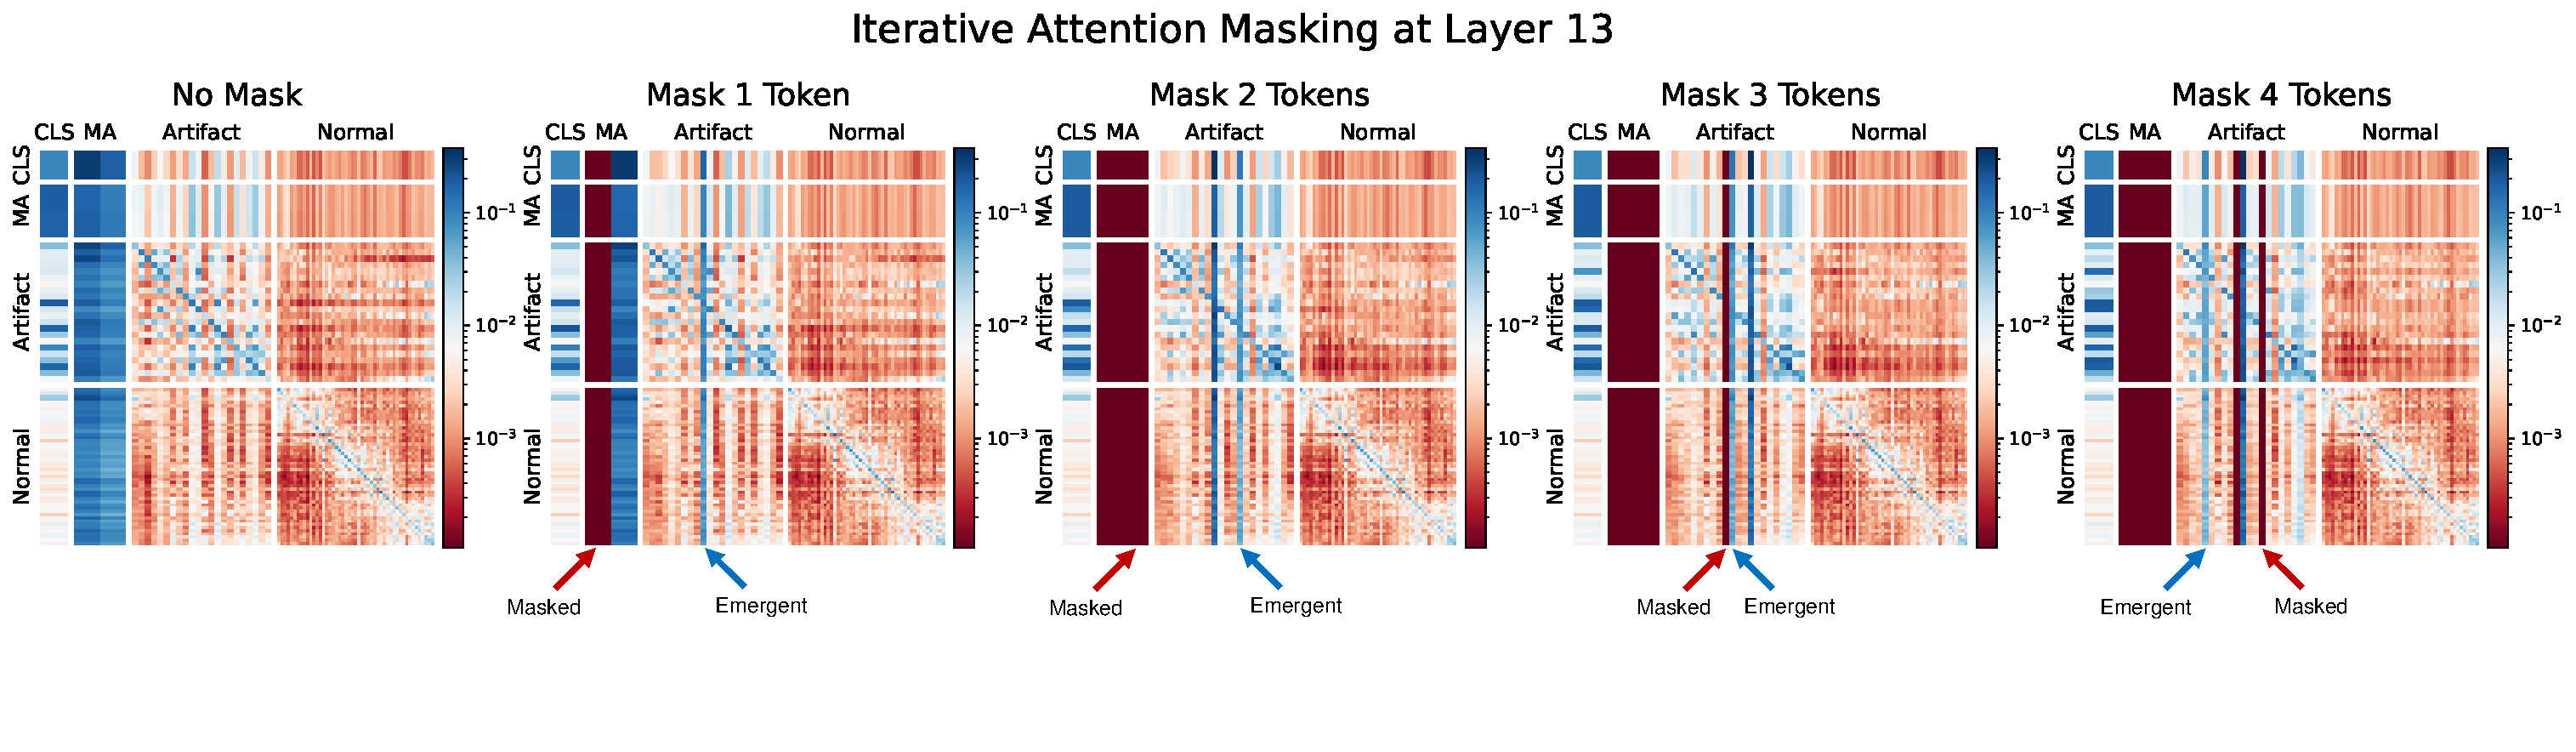
\includegraphics[width=1\linewidth]{figs/attention_iterative_removal_padded.pdf}
    \vspace{-2em}
    \caption{Each subplot depicts the result of a step in the iterative removal process for a single image in CLIP ViT L-14. The leftmost attention matrix shows that massive tokens emerge as the natural attention sinks. However, each subsequent step masks out the most prominent attention sink (indicted with the red arrow) which results in the emergence of a new attention sink as a substitute (indicated with the blue arrow).}
    \label{fig:iterative_removal}
\end{figure*}


\subsection{Non-iterative Detection of Attention Sinks}
\label{sec:artifact_classifier}

While our iterative method for extracting massive tokens is both precise and interpretable, it incurs a significant computational cost due to the need for multiple passes through the model's intermediate layers. However, in practice, massive tokens become readily identifiable shortly after their formation, as evidenced by feature visualization techniques (see Figure \ref{fig:dino_clip_artifacts}). Consequently, we can approximate the results of our iterative algorithm using traditional discrete clustering methods—such as Multi-class Spectral Clustering \cite{shi2000ncut} \cite{yang2024ncut}—to achieve a more computationally efficient, non-iterative classification of massive and artifact tokens.

